\documentclass[12pt,oneside]{book}
\usepackage{fullpage}
\usepackage{amsmath}
\usepackage{amssymb}
\usepackage{amsfonts}
\usepackage{graphicx}

\usepackage[utf8]{inputenc}
\usepackage{geometry}
\usepackage{fancyhdr}
\usepackage [english]{babel}
\usepackage [autostyle, english = american]{csquotes}


\MakeOuterQuote{"}

\rfoot{Page \thepage}
\fancyhead{}
\rhead{\thepage} 
\lhead{} 


\geometry{
 a4paper,
 total={210mm,297mm},
 left=35mm,
 right=25mm,
 top=25mm,
 bottom=25mm,
}
\linespread {1.6}





%Gummi|065|=)

\date{}
\begin{document}

%% ----------------------------------------------PAGE 1 TITLE

\begin{titlepage}
    \begin{center}
        \vspace*{1cm}
        
        {\scshape {\huge{I}\Large{NTER-PROCEDURAL} \huge{A}\Large{NALYSIS OF}\\
                   \vspace{0.1cm}
				   \huge{C}\Large{ONCOLIC } \huge{E}\Large{XECUTION}}}\\[1.5cm] % Thesis title

        
        \textit{A Thesis Submitted\\
        in Partial Fulfilment of the Requirements\\
        for the Degree of\\}
                \vspace{0.8cm}
        \textbf{\large{MASTER OF TECHNOLOGY}}\\[0.5\baselineskip]
        \textit{by}\\[0.5\baselineskip]
        \textbf{\large{Ashwini Kshitij}}\\
                \vspace{0.8cm}
        \textit{supervised by}\\
                \vspace{0.8cm}
        \textbf{\large{Dr. Subhajit Roy}}\\
        \textbf{\large{Dr. Amey Karkare}}
        \vspace{0.8cm}
        
      	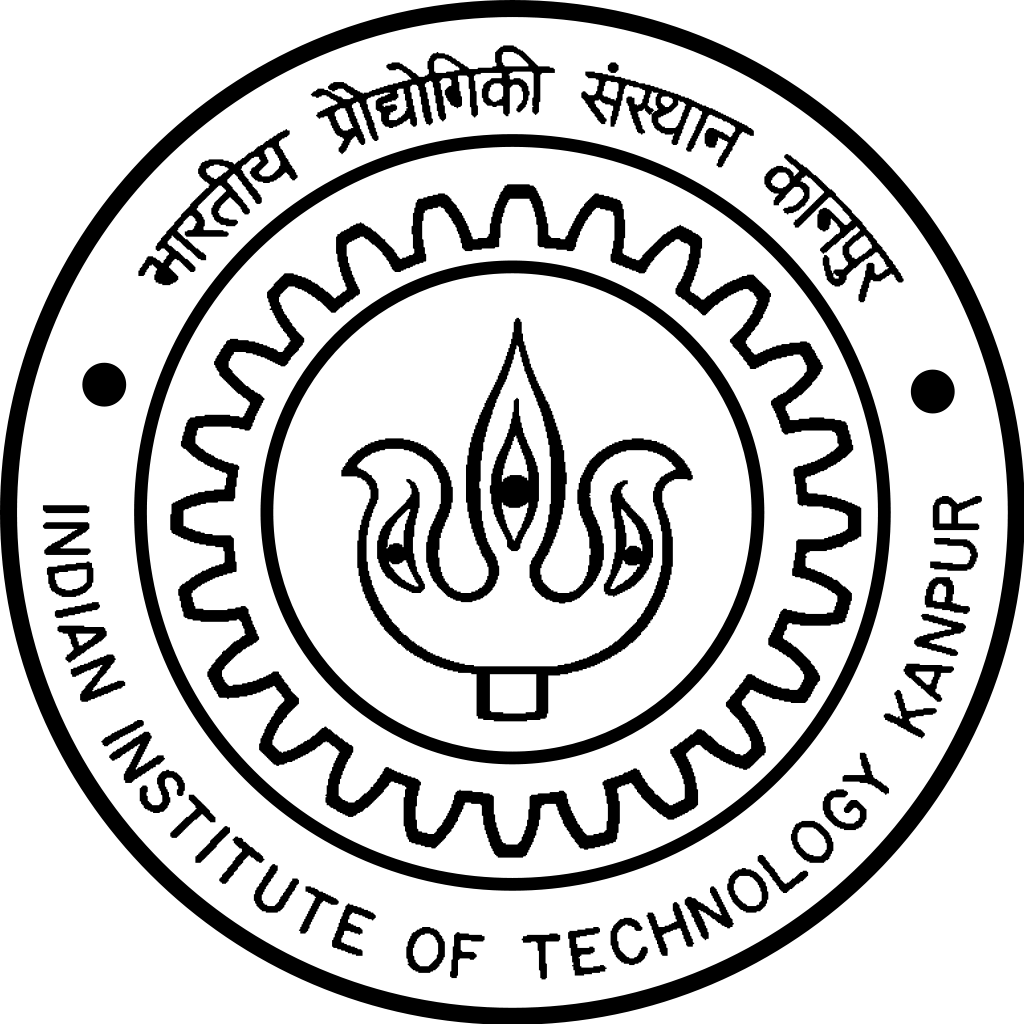
\includegraphics[width=0.25\textwidth]{iitklogo.png}
        
        \vspace{1\baselineskip}
        
        \uppercase{Department of Computer Science and Engineering\\
        \textbf{Indian Institute of Technology Kanpur}}\\
        
        \vspace{1\baselineskip}
        \textbf{June 2015}
        
    \end{center}
\end{titlepage}


%%-----------------------------------------------PAGE 2 Certificate

\frontmatter
\addcontentsline{toc}{chapter}{Certificate}
\begin{center}
\textbf{\Large{CERTIFICATE}}
\end{center}
\vspace*{3\baselineskip}
This is to certify that the work contained in this thesis entitled \textbf{\textit{"Inter-procedural analysis of Concolic Execution"}}, by \textbf{Ashwini Kshitij (Roll No. 10327165)}, has been carried out under my supervision and this work has not been submitted elsewhere for a degree.\\
\\[4\baselineskip]

  \small
  \vspace{2.0 cm}
  \begin{tabular*}{1.0\textwidth}{@{\extracolsep{\fill}} l r}
    \textbf{Dr. Subhajit Roy} 			 & 				\textbf{Dr. Amey Karkare}\\
    Assistant Professor,				 &				Assistant Professor,\\
    Department of CSE, 					 & 				Department of CSE,\\
    IIT Kanpur.							 &				IIT Kanpur.
    
  \end{tabular*}
\newpage


%%----------------------------------------------ABSTRACT
\addcontentsline{toc}{chapter}{Abstract}
\begin{center}
\textbf{\Large{ABSTRACT}}
\end{center}
\vspace {0.8 cm}

Interprocedural analysis is the cornerstone of determining precise program behavioral information. Using this technique we can avoid making overly conversative assumptions about the effects of procedures and the state at call sites. It aims at gathering informations across multiple procedures.  

\vspace {0.5 cm}

In this thesis, to extend the concept of concolic execution to interprocedural calls we instrument the function call site. For such instrumentation purposes we have used a tool called CIL. Just before the function call we set up the environment for calling the procedure which in turn enables the it follow through the symbolic execution of parameters with the control flow from caller to callee. Similarly, just after the call instruction we restore the calling environment by restoring the symbolic values.

\vspace {0.5 cm}

Modifying the symbolic execution engine to collect the interprocedural analysis information can have widepread applications in software verification and testing. We can improve the coverage of test suites that are automatically generated by intraprocedural concolic executers.   

  






\newpage

%%----------------------------------------------ACKNOWLEDGMENT
\addcontentsline{toc}{chapter}{Acknowledgement}
\begin{center}
\textbf{\Large{Acknowledgements}}
\end{center}

\vspace{1.0 cm}

I acknowledge, with gratitude, my debt of thanks to Professor Subhajit Roy for his advise and encouragement and to Professor Amey Karkare for his aid and foresight. They presented me with the opportunity to tackle interesting problems in field of Software Testing. Their patient but firm guidance was critical to successful completion of my research.  

\vspace{0.5 cm}

I appreciate the support of my friends and wingmates who always provided me with the confidence and courage to tackle even the most challenging problems. Without their help and councel, the completion this work would have been immeasurably more difficult. 

\vspace{1.0 cm}

I also want to express my sincere gratitude to \textit {\textbf {BRNS}} for encouraging our research work. Their unshaken faith in our efforts motivated me to follow through this project.

\begin{flushright}
\textbf{-Ashwini Kshitij}
\end{flushright}

\newpage

%%----------------------------------------------CONTENTS

\tableofcontents
\listoffigures
\listoftables


\mainmatter

%%---------------------------------------------CHAP 1 Intro

\chapter{Introduction}
%%\lhead{Chapter 1. \emph{Introduction}}


\hspace {0.4 cm}
Symbolic Execution has been a recipient of significant attention during the past few years. It is now considered an effective technique in generation of high coverage test suites. The idea has been discovered around three decades ago but it was after significant improvements the potential of idea is harnessed. One such important improvement was symbolic execution alongside keeping track of concrete values (concolic executic). The main advantage of this technique is that whenever constraint solving complications (like timeouts) occur during classical symbolic execution, it is alleviated using the concrete values.

More practical programs involve procedure calls. The symbolic execution goes smoothly if there are no function calls involve (\textit{intraprocedural analysis}). A function call tranfers the control from the caller to the callee. That function may very well modify the symbolic state of the variables. If we transition the symbolic state correctly through the function call, the symbolic execution will run correctly with the modified symbolic state.   

%%----------------------------------------------MOTIVATION

\section{Motivation}
\textit{Intraprocedural Analysis} is performed at one procedure at a time. It is simple and conservative. But almost all real world programs involve procedural calls. This poses problem for techniques such symbolic execution since they dont know how the procedure is going to modify the symbolic state. This brings us to the need of extending our analysis techniques to prgrams with functions and procedures.

%%----------------------------------------------PROBLEM STATEMENT

\section{Problem Statement}
This thesis aims to provide a method that can capture the transformation of the symbolic state of the inputs when the program goes through a function call. Our implementation uses inbuilt concolic execution engine for the purpose. But the engine cannot handle a procedure call. At the call site, the symbolic value is reset to "start state" instead of modifying it as per the operations performed on it by the callee function. Merging our approach with this concolic engine will increase the accuracy the tool. 

\begin{figure}[htbp]
\centering
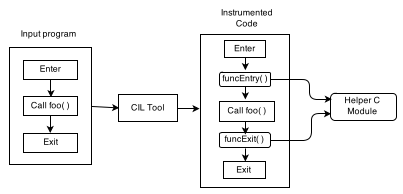
\includegraphics[scale=1]{module3.png}
\caption{Basic Module}
\end{figure}

\textit{Figure 1.1} shown above gives a vague idea of what our implementation does. We are given a C program with a concolic execution engine integrated with it. Problem arises with execution when it comes across a procedure call instruction. The symbolic state of the input variables is set to default as the program does not have the ability to follow through symbolic execution from caller to callee and then back to the caller.

We aim at solving this problem by instrumenting the call site. For such purposes in our approach we have used a tool called CIL. We first set up an environment before commencing the callee procedure execution (in this case \textit{foo}). The operations for such tasks is carried out by \textit{funcEntry} function which is instrumented just before \textit{foo} is called. \textit{funcEntry} handles the mapping of symbolic and concolic values of actual parameters to formal parameters, the creation of symbolic stack (later explained in \textit{Chapter 3}).

Similarly we instrument \textit{funcExit} function just after \textit{foo} call. The task of \textit{funcExit} is to map the symbolic state of "return variable" to appropriate variable at the call site (if any) and clear the symbolic values that were generated during call and execution of \textit{foo}. It also manages the symbolic stack appropriately. The implementation of \textit{funcEntry} and \textit{funcExit} is done in C language and is defined in included C modules.

This approach ensures that symbolic execution is carried through correctly to and from the callee. The modified state of symbolic variables is in accordance with operations of concerned callee function (in our case \textit{foo}). This improves the accuracy and correctness of the test suite generation in our tool.  

%%----------------------------------------------CONTRIBUTIONS

\section {Contributions}
In this thesis we have accomplished the following:
\begin{itemize}
  \item Designed an approach to apply inter-procedural analysis to concolic execution. 
  \item Application of IP analysis to improve the automatic test case generation using concolic testing.
  \item Dynamic support to handle recursive procedure calls. 
\end{itemize}

%%----------------------------------------------ORGANISATION OF THESIS

\section {Organisation of thesis}
A brief summary of the contents of other chapters of this thesis are as follows.\\

\textbf{Chapter 2} deals with the concepts which are necessary to understand the thesis. Concolic execution is introduced and its advantages over classical symbolic execution and random testing. An overview of approaches in interprocedural analysis like Function Inlining and Call String have also been discussed in this chapter. We have also briefly mentioned the related work that has been done in this field. \\

\textbf{Chapter 3} discusses our implementation in a detailed manner. Some terminology has been introduced to explain techniques employed in our work. But mostly the chapter pertains to the relevant algorithms designed to accomplish the aim of this thesis and how it should improve the scalability and accuracy of concolic IP analysis.\\

\textbf{Chapter 4} contains the experimental results and their analysis after we run our modified tool on a set of standard benchmark programs. Analysis in done in terms of coverage improvement and runtime of the tool.\\

\textbf{Chapter 5} sheds light on future work and modifications that can be done to improve the accuracy and performance of the approach discussed in this thesis.

%%----------------------------------------------CHAPTER 2 : BACKGROUND

\newpage
\chapter{Background}

%%----------------------------------------------INTERPROCEDURAL DATAFLOW ANALYSIS

\section {Intraprocedural Data-flow Analysis}
This is a technique which is broadly defined as gathering of information across multiple procedures (typically over the entire program). Procedure call poses barrier to program analysis. Its aim is to avoid making conservative assumpions about the effect of procedures and the state at call sites.

Interprocedural analysis is more demanding and challenging than intraprocedural analysis; here we need to take into account the call-return and parameter passing mechanisms, local variable of the function and function recursion (can be unbounded). In some cases the called procedure is known only in run-time like with function pointers or with virtual functions. 

\textbf{Application :} Interprocedural analysis (IPA) enables the compiler to optimize across different files (whole-program analysis), and can result in significant performance improvements by removing spurious data dependencies. Integrating IPA with intraprocedural concolic execution will help anticipate the precise behavior of function calls on the symbolic state of the variables.

%%----------------------------------------------FUNCTION INLINING 

\subsection {Function Inlining}
One of the approaches is \textit{function inlining} which is the simplest and most widely used approach for accurate interprocedural symbolic execution. We simply use the copy of procedure's Control Flow Graph (CFG) at each call site. This leads to function being re-analyzed at every call site. This is can be avoided using \textit{function summaries}. They are implemented by merging all states at the function exit after computing an intraprocedural path constraint in terms of function input.\\ 

\begin{figure}[htbp]
\centering
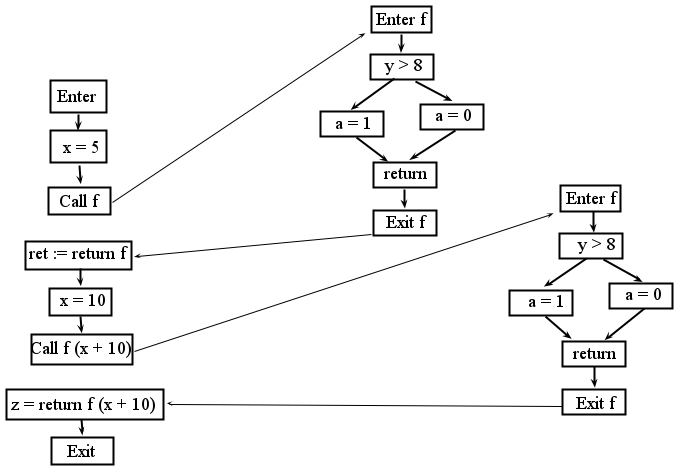
\includegraphics[scale=0.5]{inlineCFG.png}
\caption{Function Inlined}
\end{figure}

This technique does not require function calling overhead. It also saves the overhead for manipulating function stack. In increases locality of reference by utilizing instruction cache.

But there are significant \textit{drawbacks} with this approach. Firstly, the performance overhead will increase if the the code size of the inlined function is increased. The caller function may not fit on the cache causing high cache miss rate. Similarly if there are too many function calls involved, inlining maybe expensive since it will cause an exponential increase in the size of the CFG.

Secondly it is also going to create problems in the recursive procedures. Same can be said more generally for any scenario where there are cycles in the call graph. So basically function inlining has scalability issues pertaining to code size. Lastly, procedure inlining is only possible if the target of the call is known. Hence it will not be possible if call is via a pointer or is "virtual".

%%----------------------------------------------CALL STRING APPROACH

\subsection {Call String Approach}
In another IP analysis we observe the CFG's of all the procedures. In this technique,
\begin{itemize}
\item When we encouter a function call we interpret it as a goto from the call intruction to the first instruction of the procedure.
\item Interpreting every return statement like a goto to the instruction following each call site that invoked that procedure (\textit{Non-Deterministic}).
\end{itemize}
Using this method non-deterministically will allow non feasible paths in our analysis which will cause loss of accuracy. In a better approach called "Call String" we keep track of the where we came from, that is, the context of the call and where to return. To do this we maintain a "string" that simulates a call stack. A feasible path is a control flow path that is generated in accordance with the stack regime. A perfect solution is keep record of the whole stack. This concept is easy and intuitive according to which every return jumps to the instruction that's immediately after the call site which corresponds to that particular function call. By adding the context of the call to the information in the state we can overcome the problem of passing through invalid paths.\\

\begin{figure}[htbp]
\centering
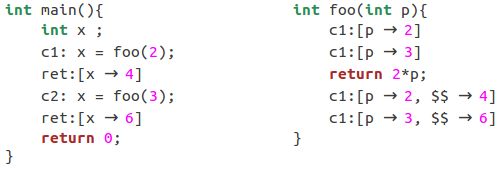
\includegraphics[scale=0.6]{callString.png}
\caption{Example : Call String}
\end{figure}  
 
Every procedure records their state information when they are invoked. Let us consider the program in \textit{Figure 2.2}. Here the labels \textit{c1} and \textit{c2} are saved in the state information of \textit{foo}. This is so that \textit{p} gets differentiating values every time function \textit{foo} is called. Another reason to save the labels is because they help in figuring out the respective return values of call \textit{c1} (\$\$ $\rightarrow$ 4) and \textit{c2}(\$\$ $\rightarrow$ 6).

Implementing this algorithm is efficient for small strings. Problem arises when call string generated is large since we can keep track of only limited number of strings. This poses a limitation on the depth of function calls.

%%----------------------------------------------CONCOLIC TESTING


\section {Concolic Testing}

One popular approach for automated software testing is \textit{random testing} which involves subjecting the program to be tested to a stream of random data. It is fast but it can find only basic bugs like program crashes, code assertions or memory leaks. But it is not always possible to employ this technique specially when working with binaries since it is very difficult to figure out the expected inputs. The code coverage generated by random data is very low.\\

A more deliberate approach can be used by merging symbolic execution with concrete execution (\textit{concolic execution}) and then using a an SMT-solver (like Z3) to generate test inputs. This method is called \textit{Concolic testing}. It is much more efficient than symbolic execution. To understand why let us assume that our costraint solver cannot handle non-linear constraint. Then a path constraint with \textit{cubic or modulo} function involved cannot be solved and symbolic execution will be stuck. Similar problem arises when we encounter a closed third party library function say \textit{increment()}. It doesn't know how to modify the symbolic state according to the behavior of that function. For such cases the test cases cannot be generated by classical symbolic execution. Concolic Tesing addresses these limitations and resolves situations like above by replacing the symbolic values by their concrete values so that the resulting constraint can be solved by the constraint solvers.\\

The algorithm involves initialting the inputs with randomly generated values. The program is executed and during the execution, on every conditional branch statement program collects symbolic path constraints on inputs. Symbolic constriants are essentially a set of logical constriants on input data. New program path is directed and executed by \textit{negating/flipping} the last condition of the path constraint. This is done until all the feasible program paths are explored. To get the intuition, let us consider the program in \textit{Figure 2.2} for concolic testing.  

\newpage

\begin{figure}[htbp]
\centering
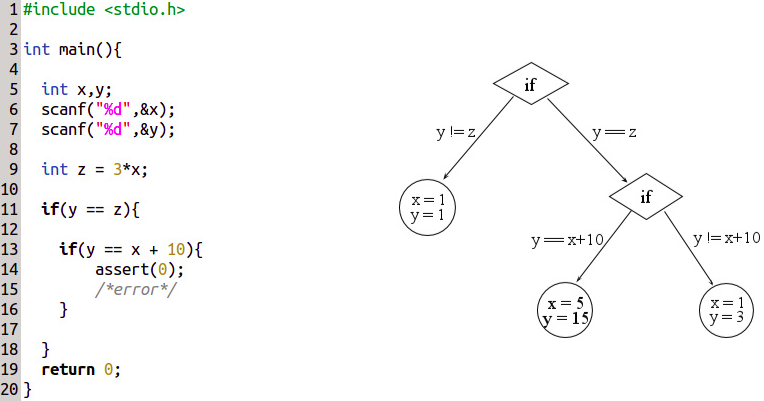
\includegraphics[scale=0.5]{conjoined4.png}
\caption{Concolic Testing}
\end{figure}

The program input variables are assigned random concrete values, say \textit{x = 1} and \textit{y = 1}. The program runs and line 11 is executed. Path condition generated is :

\begin{equation}
\neg(y == 3x)
\end{equation}

Now we negate the last condition in path constraint (PC has only one condition in this case) to execute an alternate path. So the new path constraint generated is :

\begin{equation}
y == 3x
\end{equation}

which is examined by a SMT solver to generate the new input data. Out of many different possible values for equation \textit{2.2} solver picks say \textit{x = 1} and \textit{y = 3} which should explore a different path than before. The program runs on these new inputs and generates a new path condition :

\begin{equation}
(y == 3x) \wedge \neg(y == x + 10)
\end{equation}

Like previously we negate the last condition of the path constraint to generate condition for new path exploration.
So we pass on the following constraint to solver to generate new inputs

\begin{equation}
(y == 3x) \wedge (y == x + 10)
\end{equation}

Let the new inputs generated be \textit{x = 5} and \textit{y = 15} we will lead to the execution of line 13 and consequently line 14 which will hit the error or any other unexpected behavior. Since there are no more paths left to explore, the algorithm will terminate generating a set of input data for complete path coverage of this program.

%%----------------------------------------------RELATED WORK

\section {Related work}

%%----------------------------------------------SUMMARY BASED ANALYSIS

\subsection {Summary-based Analysis}
New techniques have been invented that compute procedure summaries for performing an interprocedural analysis of programs. In summary-based context-sensitive analysis we create "summary" which is succinct description of the observable behavior of each procedure. The purpose of this approach is to prevent renanalysing the behavior of same procedure when there are invoked at each call site.

The representation of every has a single eantry point. The analysis is divided into following two phases:
\begin{itemize}
  \item \textit{Buttom-Up} : To summarize the effects of a procedure, transfer function is computed.
  \item \textit{Top-Down} : To propogate the caller information to compute callee result.
\end{itemize}

%%----------------------------------------------DART

\subsection {DART}
DART is an abbreviation for "\textit{Directed Automated Random Testing}" which is a tool for automated test case generation developed by \textit{Patrice Godefroid, Nils Klarlund} and \textit{Koushik Sen}. It utilizes the concept of concolic execution and is comprised of the following techniques :
\begin{itemize}
 \item \textit{Automated} extraction of program interface from source code.
 \item \textit{Random testing} the program interface by generating a test driver. 
 \item Dynamic generation of test cases to \textit{direct} alternate program execution path.
\end{itemize}

\newpage

%%----------------------------------------------CUTE

\subsection{CUTE}
CUTE stands for "A Concolic Unit Testing Engine for C" which also addresses automatic test case generation with memory graphs as inputs. This tool is developed by \textit{Koushik Sen}, \textit{Darko Marinov} and \textit{Gul Agha}. It is similar to DART, thereby employs concolic testing technique. It resolves some of the limitations of DART and aims at testing real-world examples of C code.

It provides a method for representing and solving approximate pointer contraints to generate test inputs. The symbolic model being used is more powerful and the theorm solver is both more powerful and is built to be efficient in this system. As opposed to what DART does, CUTE does not automatically extract program interface but lets user decide relation among functions and their preconditions. The work also shows exactly how it made approximations and trade off between speed vs. correctness and scenarios where CUTE will not work correctly.






\newpage


\chapter{Methodology}
\section{Definitions}
\section{Instrumentation}
\section{Parameter Mapping}
\section{Stack Manipulation}
\section{Return Handling}

\chapter{Experiments}
\section{Result}
\section{Comparion of Test Case Generation}
\section{Analysis}

\chapter{Conclusion}
\newpage

\addcontentsline{toc}{chapter}{Bibliography}
\begin{center}
\textbf{\Large{Bibliography}}
\end{center}

\end{document}
